% ============================================================
% CAPÍTULO 5: RESULTADOS E DISCUSSÃO
% ============================================================

\section{Resultados e Discussão}
\label{sec:results}

Este capítulo detalha a avaliação experimental do Filtro de Kalman Estendido (EKF) ao longo dos seis cenários de navegação propostos na Seção \ref{sec:methodology}. A análise fundamenta-se em métricas de acurácia posicional (RMSE e Erro Máximo), consistência estatística (NIS) e validação espacial (Taxa de \textit{Inliers}). Para avaliar a sensibilidade do algoritmo, os ensaios comparam o EKF com matrizes calibradas em contraponto a uma configuração intencionalmente descalibrada. A Tabela \ref{tab:resumo_metricas_dividida_nomes} consolida os indicadores quantitativos obtidos na simulação.

Devido a restrições de formatação, as composições gráficas completas (painéis comparativos de todas as trajetórias estimadas e históricos da métrica NIS para os seis cenários) foram alocadas no \textbf{Apêndice \ref{app:graficos_completos}}. Além disso, o código-fonte do simulador, os dados brutos e as imagens em alta resolução estão publicamente disponíveis no repositório do projeto no GitHub\footnote{Disponível em: \url{https://github.com/SauloJose/PASKalmanTraj} - Acesso em: 22 jun. 2026.}.

% ============================================================
% TABELA DE RESULTADOS 
% ============================================================

\begin{table*}[t!]
\centering
\caption{Resumo das Métricas de Desempenho do EKF (Condição Sintonizada vs. Não Sintonizada)}
\label{tab:resumo_metricas_dividida_nomes}
\small
\begin{tabular}{l *{8}{S[table-format=3.2]}}
\hline \hline
\textbf{Cenário} & {$RMSE_x$ [m]} & {$RMSE_y$ [m]} & {$E_{\max}$ [m]} & {$\mu_x$ [m]} & {$\overline{NIS}$} & {$NIS \in \text{IC}$ [\%]} & {TD [\%]} & {TI [\%]} \\ \hline
\addlinespace[1mm]
\multicolumn{9}{c}{\textbf{CONDIÇÃO SINTONIZADA (Q = 0,64$\mathbf{I_6}$; R = 0,09$\mathbf{I_4}$)}} \\ \hline
\addlinespace[1mm]
\textbf{Cenário 1} & 0,11 & 0,16 & 0,64 & +0,01 & 3,39 & 96,33 & 100,00 & 100,00 \\
\textbf{Cenário 2} & 0,13 & 0,18 & 0,58 & -0,00 & 3,86 & 95,84 & 100,00 & 96,88 \\
\textbf{Cenário 3} & 0,12 & 0,14 & 0,58 & +0,00 & 3,34 & 96,58 & 100,00 & 100,00 \\
\textbf{Cenário 4} & 0,11 & 0,15 & 0,58 & +0,01 & 3,34 & 97,17 & 100,00 & 100,00 \\
\textbf{Cenário 5} & 0,11 & 0,16 & 0,57 & +0,00 & 3,49 & 96,58 & 100,00 & 100,00 \\
\textbf{Cenário 6} & 0,17 & 0,34 & 2,62 & +0,01 & 3,40 & 95,19 & 90,00  & 100,00 \\ \hline
\addlinespace[1mm]
\multicolumn{9}{c}{\textbf{CONDIÇÃO NÃO SINTONIZADA (Parâmetros Descalibrados)}} \\ \hline
\addlinespace[1mm]
\textbf{Cenário 1} & 0,23 & 0,34 & 0,75 & +0,01 & 6,76  & 80,25 & 100,00 & 10,08 \\
\textbf{Cenário 2} & 0,60 & 0,82 & 2,24 & -0,02 & 24,07 & 49,48 & 100,00 & 28,07 \\
\textbf{Cenário 3} & 0,16 & 0,20 & 0,79 & +0,00 & 23,85 & 26,75 & 100,00 & 97,25 \\
\textbf{Cenário 4} & 0,14 & 0,20 & 0,74 & +0,01 & 25,50 & 22,67 & 100,00 & 93,83 \\
\textbf{Cenário 5} & 0,15 & 0,21 & 0,73 & +0,00 & 24,14 & 26,08 & 100,00 & 96,25 \\
\textbf{Cenário 6} & 0,17 & 0,33 & 2,62 & +0,01 & 31,67 & 15,56 & 90,00  & 71,76 \\
\hline \hline
\multicolumn{9}{l}{\scriptsize \textit{Cenários:} 1: Circular; 2: Quadrada; 3: Tang. Hiperbólica; 4: Lemniscata; 5: Aleatória; 6: Oclusão.} \\
\multicolumn{9}{l}{\scriptsize \textit{Nota:} Limites bicaudais do NIS a $95\%$ de confiança para 4 G.L. são $[0,484; 11,143]$. TD: Taxa de Detecção; TI: Taxa de \textit{Inliers}.}
\end{tabular}
\end{table*}

% -------------------------------------------------------------
\subsection{Interface Gráfica e Ambiente de Simulação}
\label{subsec:gui_interface}

A Figura \ref{fig:gui_funcional} exibe o ambiente de simulação desenvolvido para este estudo. A interface gráfica integra a renderização espacial da arena, a telemetria das posições estimadas face ao \textit{ground truth} e os painéis de monitoramento temporal de RMSE e NIS. Essa estrutura permite a manipulação direta das matrizes de covariância $\mathbf{Q}$ e $\mathbf{R}$, viabilizando a análise empírica do impacto da calibração nas elipses de incerteza do filtro.

\begin{figure*}[htpb]
    \centering
    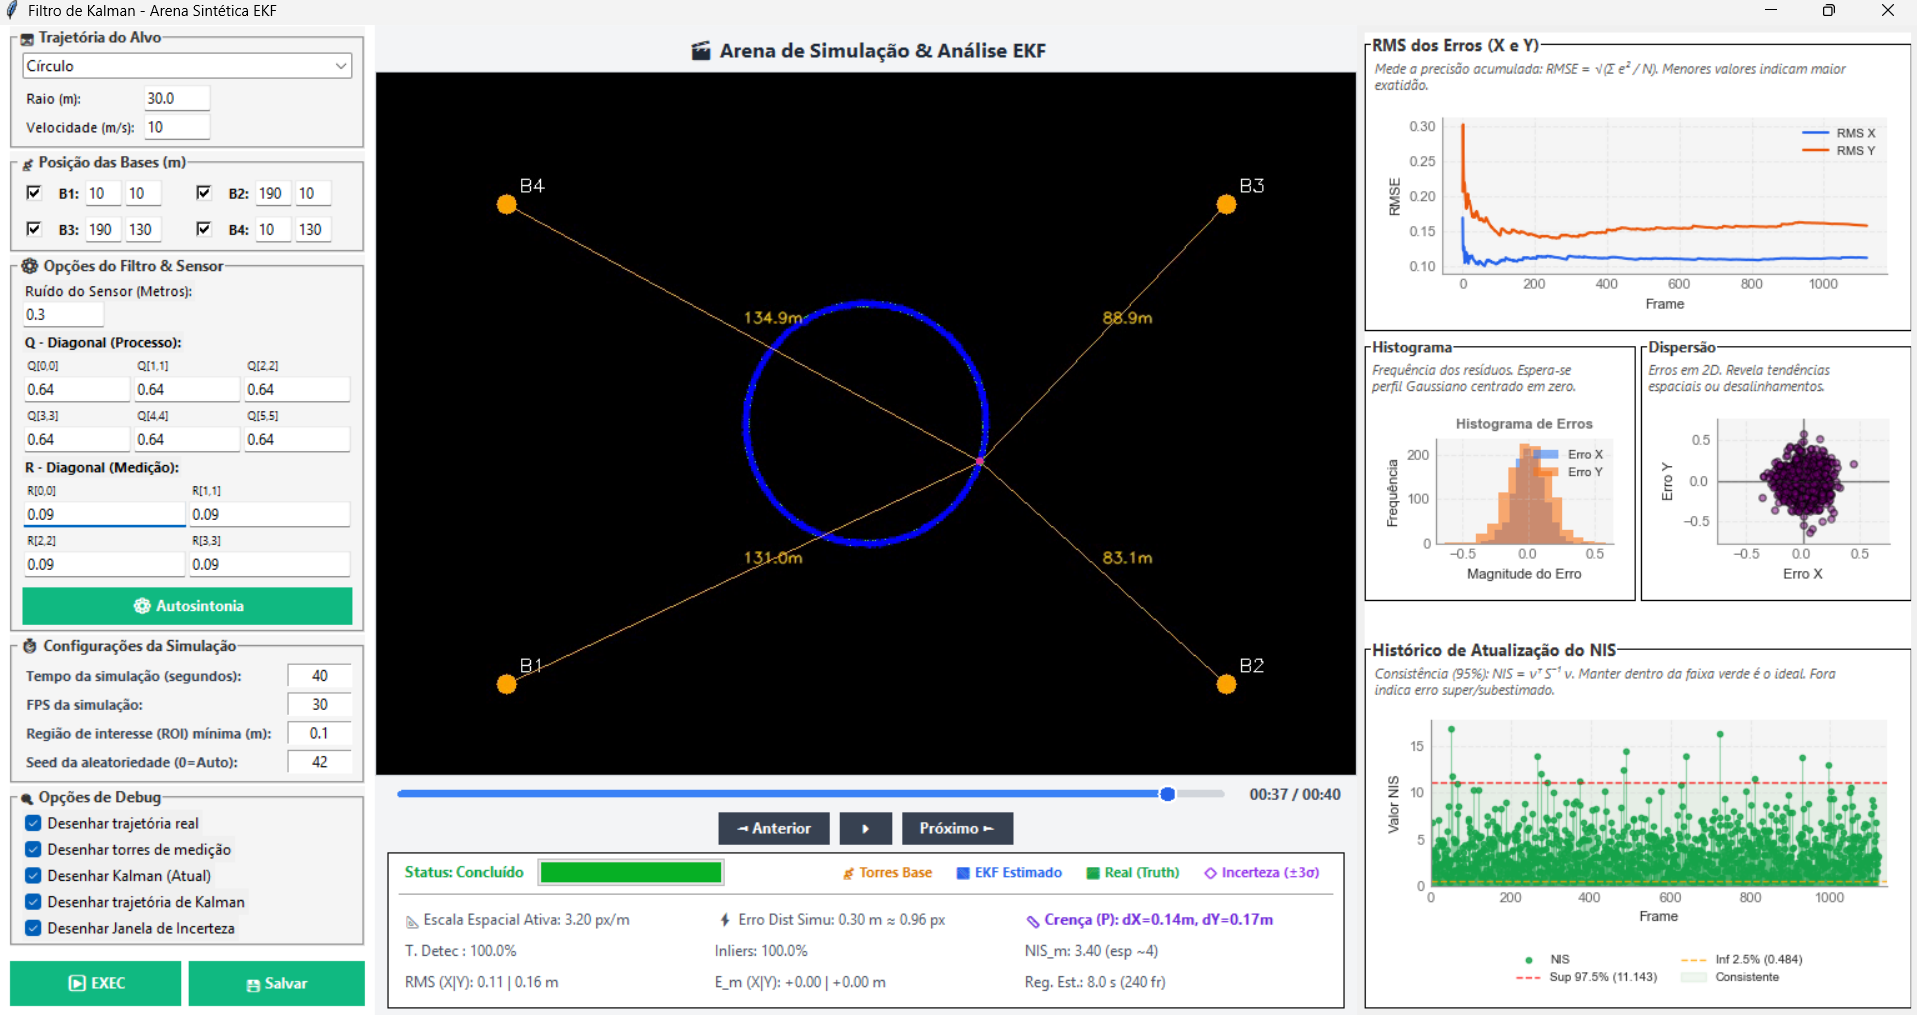
\includegraphics[width=0.9\linewidth]{Figuras/diagrams/Bases.png}
    \caption{Ambiente gráfico desenvolvido em Python. O painel central exibe a cinemática do alvo, ladeado pelos controles de simulação à esquerda e gráficos de monitoramento temporal à direita.}
    \label{fig:gui_funcional}
\end{figure*}
% -------------------------------------------------------------

\subsection{Análise de Acurácia Posicional e Distribuição de Erros}
\label{subsec:accuracy_analysis}

A parametrização do EKF apresentou correlação direta com a mitigação do ruído de observação. Conforme os dados consolidados na Tabela \ref{tab:resumo_metricas_dividida_nomes} e as trajetórias detalhadas no Apêndice \ref{app:graficos_completos}, a configuração sintonizada manteve o $\text{RMSE}_x$ e o $\text{RMSE}_y$ em níveis sub-métricos estritos, com erros em $X$ variando entre $0{,}11$\,m e $0{,}13$\,m, e em $Y$ entre $0{,}14$\,m e $0{,}18$\,m nos cenários de visibilidade total. No Cenário 2 (Trajetória Quadrada), caracterizado por descontinuidades severas de aceleração ortogonal nos vértices, a sintonia correta demonstrou robustez ao conter o Erro Máximo Absoluto em $0{,}58$\,m. Em contrapartida, a configuração não sintonizada sob regime lento ($Q=0{,}01; R=0{,}10$) falhou em acompanhar as transições abruptas, resultando em um salto do RMSE para $0{,}60$\,m em $X$ e $0{,}82$\,m em $Y$, além de registrar um pico de erro máximo de $2{,}24$\,m devido ao atraso de fase clássico.

A evolução temporal dessa métrica é detalhada na Figura \ref{fig:rmse_temporal}, onde a curva de erro da condição calibrada permanece estável e contida dentro da margem operacional prevista.

\begin{figure}[htpb]
    \centering
    
\includegraphics[width=0.9\linewidth]{Figuras/C2/sintonizado/simulacao_quadrado_2_rms.png}
    \caption{Evolução temporal do RMSE (Cenário 2). A estabilidade da curva reflete a consistência do filtro quando devidamente sintonizado frente a manobras evasivas.}
    \label{fig:rmse_temporal}
\end{figure}

Para aprofundar a avaliação do comportamento estatístico do estimador, a Figura \ref{fig:distribuicao_erros} apresenta o comportamento estocástico dos resíduos de predição. Nos gráficos de dispersão e histogramas associados à condição sintonizada, nota-se que os erros de estimação em X e Y se distribuem assintoticamente como uma normal bivariada, com viés médio estatisticamente nulo ($\mu_x \approx -0{,}00$\,m no cenário do quadrado). Quando a sintonia falha, a distribuição perde a sua característica gaussiana e exibe caudas pesadas ou dispersões deslocadas, refletindo o descompasso geométrico e o atraso de fase na estimação dos estados.

\begin{figure}[htpb]
    \centering
    
\includegraphics[width=0.9\linewidth]{Figuras/C2/sintonizado/simulacao_quadrado_5_hist.png}
    \vspace{1mm}
    \\{\small (a) Condição Sintonizada}
    \vspace{6mm}
    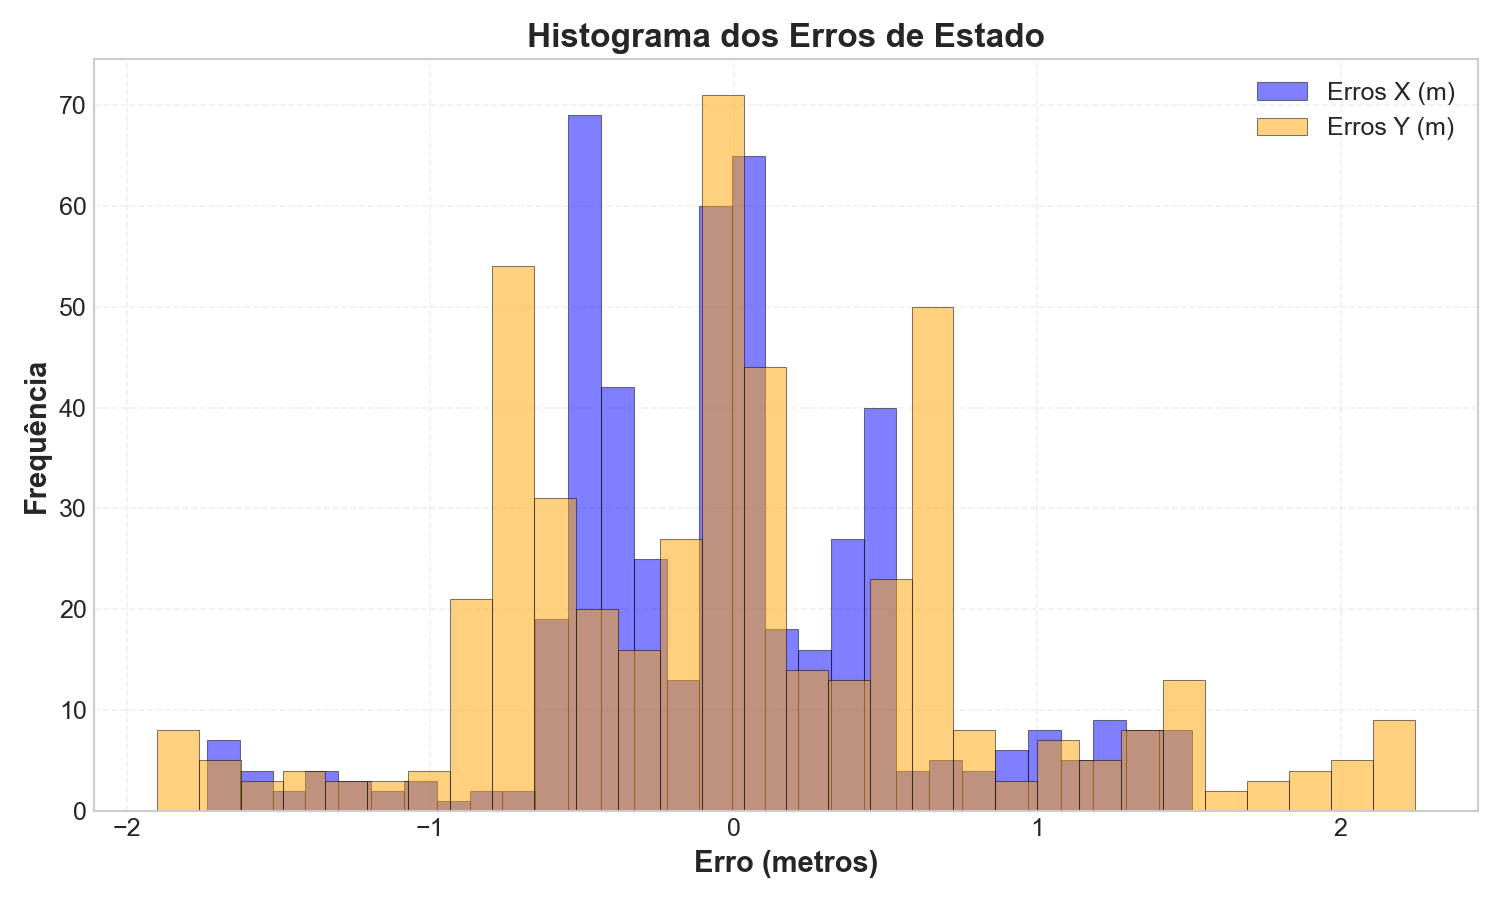
\includegraphics[width=0.9\linewidth]{Figuras/C2/nsintonizado/simulacao_quadrado_5_hist.png}
    \vspace{1mm}
    \\{\small (b) Condição Não Sintonizada}
    \caption{Histogramas e dispersão dos erros de predição (Cenário 2). Em (a), a condição sintonizada converge para uma distribuição normal centrada no zero. Em (b), a ausência de calibração induz dispersão irregular e acúmulo de erros de fase.}
    \label{fig:distribuicao_erros}
\end{figure}

\subsection{Consistência Estatística e Monitoramento do NIS}
\label{subsec:nis_analysis}

A coerência entre a incerteza teórica calculada pelo filtro e os resíduos de inovação reais foi avaliada por meio da estatística \textit{Normalized Innovation Squared} (NIS). Para o modelo rastreado por quatro torres ativas (4 graus de liberdade), a esperança teórica do NIS é exatamente $\mathbb{E}[NIS] = 4{,}0$. O limite crítico superior bicaudal para um nível de confiança de $95\%$ situa-se em $\chi^2_{0.975, 4} = 11{,}143$.

Como ilustra a Figura \ref{fig:nis_evolucao} e os dados da Tabela \ref{tab:resumo_metricas_dividida_nomes}, o EKF sintonizado demonstrou alto equilíbrio e consistência estatística. Os valores médios operacionais ($\overline{NIS}$) flutuaram estavelmente entre $3{,}34$ e $3{,}86$, aproximando-se com rigor do valor teórico esperado de $4{,}0$. As taxas de violação do limite superior permaneceram estritamente controladas (entre $0{,}75\%$ e $2{,}29\%$), validando estatisticamente a matriz de covariância do erro de estimação $\mathbf{P}$.

Por outro lado, o perfil não sintonizado expôs dois comportamentos patológicos distintos: nos cenários de subestimação drástica do ruído de leitura ($R=0{,}01$ nos Cenários 3 a 6), o filtro operou em regime severamente otimista. A média do NIS disparou (atingindo $31{,}67$ no Cenário 6), com taxas de violação do limite crítico que superaram $84\%$. Nos cenários com superestimação de $R$ combinada com redução de $Q$ (Cenários 1 e 2), o filtro tendeu à lentidão e perda de reatividade, acumulando inovações elevadas que inflaram o $\overline{NIS}$ para $24{,}07$ no Cenário 2, estourando o limite em mais de $50\%$ das amostras.

\begin{figure}[htpb]
    \centering
    
\includegraphics[width=0.9\linewidth]{Figuras/C3/sintonizado/simulacao_tangente_hiperbólica_4_nis.png}
    \caption{Comportamento temporal da métrica NIS. A calibração adequada mantém o parâmetro próximo à média teórica ($4,0$) e abaixo do limite crítico superior ($11,14$).}
    \label{fig:nis_evolucao}
\end{figure}

\subsection{Região de Confiança e Taxa de Inliers}
\label{subsec:inliers_analysis}

A Taxa de \textit{Inliers} (TI) quantificou a porcentagem de frames em que o erro real de posicionamento esteve contido dentro da elipse de confiança calculada pelo filtro. Nos cenários sintonizados, em decorrência da calibração exata das covariâncias, a TI apresentou desempenho ótimo, cravando $100{,}00\%$ nas trajetórias suaves (Cenários 1, 3, 4, 5 e 6) e mantendo-se em patamar seguro de $96{,}88\%$ na severa geometria do quadrado. Isso assegura que as elipses geradas pelo estimador refletem de forma fiel a dispersão espacial do erro. Na condição descalibrada dos Cenários 1 e 2, o estreitamento incorreto das elipses combinado ao atraso físico da trajetória fez a região de confiança colapsar, derrubando a TI para níveis críticos de $10{,}08\%$ e $28{,}07\%$, respectivamente.

\subsection{Resposta Transitória sob Oclusão (Cenário 6)}
\label{subsec:occlusion_analysis}

O Cenário 6 validou a estabilidade do algoritmo em malha aberta ao impor uma janela de oclusão temporária de sinal, reduzindo a Taxa de Detecção (TD) global para $90\%$. A Figura \ref{fig:analise_oclusao} detalha o intervalo de interrupção das medições. A modelagem cinemática consistente permitiu que a propagação de estados estimasse a posição puramente preditiva com base nas últimas velocidades calculadas. Embora o afastamento temporário do sinal tenha expandido o erro máximo absoluto para $2{,}62$\,m no ápice da oclusão, o sistema evitou o colapso numérico e restabeleceu a convergência sub-métrica imediatamente após a reconexão com as balizas, mantendo um RMSE global controlado de $0{,}17$\,m em $X$ e $0{,}34$\,m em $Y$.

\begin{figure}[htpb]
    \centering
    
\includegraphics[width=0.9\linewidth]{Figuras/C6/sintonizado/simulacao_oclusão_1_traj.png}
    \caption{Recorte do Cenário 6 sob oclusão temporária. O EKF propaga a cinemática em malha aberta sem divergência crítica.}
    \label{fig:analise_oclusao}
\end{figure}